\section{SMITER MPI Developers Manual}
\label{loc:smiterDevMan}

\subsection{Structure}
The MPI changes to the smiter code consist of 3 basic additions to the existing smiter package.

\begin{itemize}
\item {\tt powcal} decomposition over track starting locations
\item Broadcast routines to communicate data both within {\tt powcal} and between the {\tt smiter} steps
\item New {\tt smiter} program unit that allows the running of the smiter package as a single executable
\end{itemize}

Most MPI related code is contained in two new files, {\tt smitermpi\_m.f90} which contains all the MPI library calls and MPI related subroutines and {\tt smitermpi\_h.f90} which contains the declaration of the {\tt decomp\_t} structure (see \ref{loc:decomp_t}) and a global variable {\tt myrank\_log} which is used in limited cases to avoid adding extra arguments to existing smiter subroutines, particularly in the log files. This variable replaces {\tt myrank\_global} used in earlier versions. The smiter code uses functional and domain decomposition to allow the most efficient running of the code. The {\tt powcal} component of smiter is decomposed over the domain of track starting positions while the {\tt geoq} and {\tt hdsgen} components are decomposed functionally. The new MPI code follows the style and conventions already in place in the smiter suite of codes.

The smiter functional decomposition is part of the changes made to allow smiter to run as a single executable, combining the 3 smiter components that were previously compiled as separate executables, {\tt geoq, hdsgen} and {\tt powcal} into a single executable. Changes were made to each of the 3 smiter component source files {\tt geoq.f90, hdsgen.f90} and {\tt powcal.f90}. These files originally each contained a single program unit, these have now been altered to Fortran90 modules with the suffix {\tt \_p} to differentiate them from the other module files with suffix {\tt \_m}. Each module contains a single subroutine with the suffix {\tt \_sub} and three arguments, {\tt arg, combined} and {\tt decomp}. A program unit with the same name as the original has also been added to each file which calls only the relevant subroutine. This program unit is contained within an {\tt \#ifndef} preprocessor directive so that by default each component will compile and link as its own executable in the same way as was done previously using the relevant Makefile. In addition a new file {\tt smiter.f90} has been added to the repository along with its Makefile {\tt Makefile.smiter}. This file contains a single program unit that initialises MPI and calls each of the {\tt \_sub} subroutines corresponding to the smiter components. The control flow of this program unit can be seen schematically in figure \ref{fig:smiterControl}. A more detailed description of the {\tt smiter} program and each of the smiter components is presented below.


\begin{figure}
  \begin{center}
    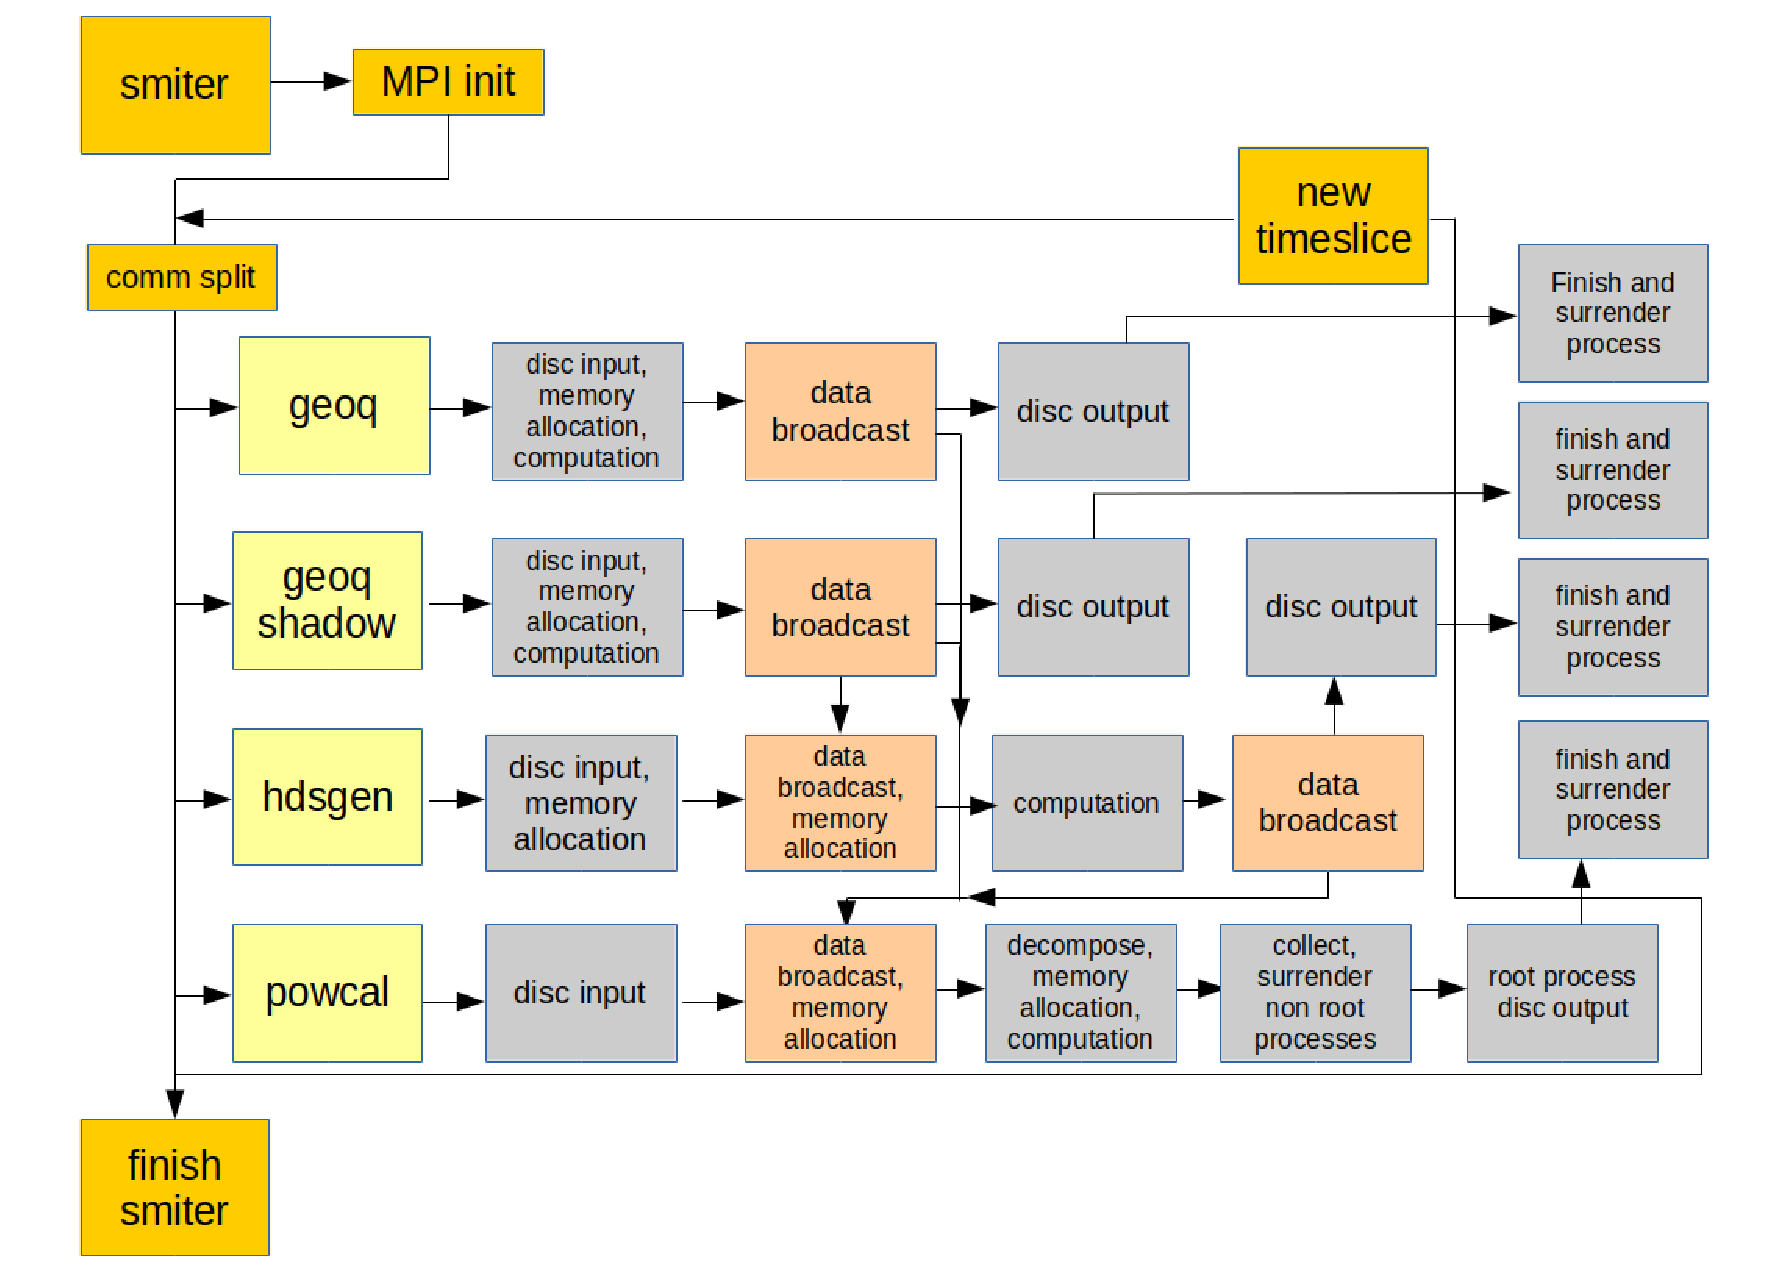
\includegraphics[width=\textwidth]{images/smiterControlFlowLS.eps}
    \caption{Control flow for the smiter when run as a single program unit. Orange refers to tasks carried out on all available processes by the smiter program unit. Yellow refers to the existing smiter program units as subroutine calls. Grey refers to calls by the subroutines. Pink indicates communication with the main smiter control flow.\label{fig:smiterControl}}
  \end{center}  
\end{figure}


\subsection{\tt smiter}
\label{loc:smiter}
The {\tt smiter} program unit controls the distribution of smiter components to available processes. Here the term component will be used to describe the 3 subroutines or program units that make up the core {\tt smiter} package, {\tt geoq, hdsgen} and {\tt powcal}. The term step will be used to describe the 4 specific calculations being carried out, {\tt geoq} shadow, {\tt geoq} results, {\tt hdsgen} and {\tt powcal}. {\tt smiter} first calls the subroutine {\tt smitermpi\_init} which initialises MPI and creates groups and communicators for all of the components to be run. The process for each component is set during initialisation and the smiter program then instructs the correct process to run each component using the {\tt decomp} structure, \ref{loc:decomp_t}. {\tt geoq} and {\tt hdsgen} are run on single processes and {\tt geoq} is run twice, once for the shadow and once for the results, different communicators are used for each of these tasks. The execution of the {\tt powcal} step is controlled by the logical {\tt powcal} in the {\tt decomp} type so that any process with {\tt powcal} set {\tt True} will call the powcal step. Data broadcasts between steps are dealt with solely by the individual components and not by the {\tt smiter} program unit. A schematic of the flow control can be seen in figure \ref{fig:smiterControl}.

In summary {\tt smiter} initially calls all 4 smiter steps which read configuration data from disk. {\tt geoq} shadow and results and the {\tt hdsgen} steps all run on a single process while {\tt powcal} runs on as many processes as are available. The {\tt geoq} shadow and {\tt geoq} results steps then run to completion. The {\tt hdsgen} step waits for a data broadcast from the {\tt geoq} shadow step and itself then runs to completion. The {\tt powcal} step then receives data broadcasts from the {\tt geoq} shadow and results steps and then waits a short time for the creation and broadcast of the Hierarchical Data Structures from the {\tt hdsgen} step. Once {\tt powcal} has completed its track evaluation the non root processes are released and powcal uses only the root process to write to disk. In practice the runtime of the full set of codes is defined by the run time of the {\tt geoq} shadow step which spends most of its runtime writing diagnostic data to disk.


\subsubsection{MPI Initialisation}
Smiter initialises MPI in the subroutine {\tt smitermpi\_init}. A duplicate of the {\tt MPI\_COMM\_WORLD} communicator is store in the {\tt commsmiter} variable in the {\tt decomp} type. This calls {\tt smitermpi\_control} which decides on the runtime behaviour and sets a series of control flags governing process assignment and data broadcasts. If 6 or less processes are available smiter will run the 3 components to completion before starting powcal as the extra cores available for {\tt powcal} improve the runtime When running on 2 cores the {\tt geoq} step and {\tt hdsgen} step are run consecutively while {\tt geoq} results is run concurrently with these. When running on 3 or more processes each step is run concurrently and data is broadcast between {\tt geoq} shadow and {\tt hdsgen}. In the case where 7 or more processes are available {\tt powcal} starts as soon as data is available from the {\tt geoq} and {\tt hdsgen} components. {\tt smitermpi\_control} then calls {\tt smitermpi\_decomp} which create groups and communicators for each of the steps, see \ref{loc:comms} for a description of these communicators.

{\tt powcal} domain decomposition is not carried out in {\tt smiter} but instead in the {\tt powcal} component using the subroutine {\tt powcalmpi\_decomp}.

\subsubsection{Communicators}
\label{loc:comms}
At initialisation smiter creates a set of groups and communicators for each individual step and for communication between steps. This is carried out using the MPI routines {\tt MPI\_Group\_incl,\tt MPI\_Group\_excl} and {\tt MPI\_Group\_union}. Table \ref{tab:comms} shows the members and purpose of each communicator when running as a single executable. When powcal is running on all processes or as a standalone executable all communicators are set to {\tt commpowcal}.

\begin{table}
  \begin{center}
    \begin{tabular}{ | c | c | c | }
      \hline
      Communicator  &  Members & Purpose \\
      \hline
      {\tt commsmiter}   & All processes & Copy of {\tt MPI\_COMM\_WORLD} \\ \hline
      {\tt commpowcal}   & Processes running {\tt powcal} & Control of powcal decomposition   \\ 
                         &                                & and broadcasts within powcal      \\ \hline
      {\tt commgeoqshad} & Union of {\tt geoq} shadow     & Broadcasts from {\tt geoq} shadow \\
                         & and powcal processes           & to {\tt powcal}                   \\ \hline
      {\tt commgeoqres}  & Union of {\tt geoq} results    & Broadcasts from {\tt geoq} results \\
                         & and {\tt powcal} processes     & to {\tt powcal}                   \\ \hline
      {\tt commhdsgen}   & Union of {\tt hdsgen}          & Broadcasts from {\tt hdsgen}    \\
                         & and {\tt powcal} processes     & to {\tt powcal}   \\ \hline
      {\tt commshadhds}  & Union of {\tt geoq} shadow     & Broadcasts from {\tt geoq} shadow \\
                         & and {\tt hdsgen} processes     & to {\tt hdsgen} \\
      \hline
    \end{tabular}
    \caption{Communicators stored in the {\tt decomp} type used for smiter control.\label{tab:comms}}
  \end{center}
\end{table}

\subsubsection{Running {\tt smiter}}
\label{loc:runningSmiter}
The single executable version of smiter now takes 4 input files on the command line, one for each step. The {\tt smiter} program has not been included in the existing smiter execution scripts and so in order in run the directory structure usually created by these scripts must exist. This consists of 4 directories, {\tt S, G, H, P}, each containing the relevant {\tt .ctl} control file used in the original smiter code. To run with MPI the new {\tt smiter} executable is run from the directory above this with the command

{\tt > mpiexec -np 4 smiter S/<shadow>.ctl G/<results>.ctl H/<hdsgen>.ctl P/<powcal>.ctl}

Using the appropriate configuration files. As smiter runs in the top directory a small change is needed to the input files in that the paths in the {\tt \&inputfiles} namelist need to have the {\tt '../'} removed, e.g. {vtk\_input\_file='../S/jetbean\_geoqm.vtk'} becomes {vtk\_input\_file='S/jetbean\_geoqm.vtk'}. The geometry and equilibrium input files then need to be added to the top directory or the paths in the {\tt .ctl} input files changed to include the releveant directory, e.g. {\tt vtk\_input\_file='jet\_divertor.vtk'} becomes  {\tt G/vtk\_input\_file='jet\_divertor.vtk'}.


\subsection{{\tt smiter} components common properties}
There are several common changes to the three smiter components. Each component now consists of a module, {\tt geoq\_p, hdsgen\_p, powcal\_p} and a program unit with the same name as the original code, {\tt geoq, hdsgen, powcal}. The program unit is within a preprocessor directive {\tt \#ifndef COMBINED} so that when the original Makefile is used the the program unit is seen. However when the preprocessor flag COMBINED is set these program units are not visible by the compiler and only the module within the file is compiled. The {\tt \_p} modules contain a single subroutine with the suffix {\_sub} i.e. {\tt geoq\_sub, hdsgen\_sub, powcal\_sub}. 

The component subroutines take three arguments, {\tt integer arg, logical combined} and {\tt decomp\_t decomp}, see \ref{loc:decomp_t} for details of the {decomp\_t} derived type. The integer {\tt arg} is used as input to the {\tt get\_command\_arg} subroutine call and sets the number of the command line argument to be read at runtime. The logical {\tt combined} notifies the subroutine that it is being run as part of the single {\tt smiter} executable and enables broadcasts to other components as well as other small changes to the runtime behaviour of each code. The {\tt decomp} argument contains the MPI decomposition information that is initialised in the {\tt smiter} program unit. When the {\tt powcal} component is run as a standalone executable the {\tt decomp} type is initialised by powcal program unit instead of smiter. When {\tt geoq} and {\tt hdsgen} are rune standalone the decomp type is declared in the program unit but is not initialised as these code only run on a single core.

\subsection{\tt geoq}
\label{loc:geoq}
Apart from the common changes described previously there is only a further single line change to the {\tt geoq.f90} file. If the input argument {\tt combined} is True a call is made to a new routine {\tt geoq\_bcast} which is located in the file {\tt geoq\_m.f90}. This routine broadcasts relevant data to the {\tt powcal} and {\tt hdsgen} steps using bcast routines described in \ref{loc:bcast}. {\tt geoq\_bcast} operates differently depending whether {\tt geoq} is generating the results or shadow geometry.

When generating results geometry, broadcasts are made to the {\tt powcal} step through a call to {\tt bcast\_powcal} followed by a call to {\tt bcast\_position} both using the {\tt commgeoqres} communicator. The call to {\tt bcast\_position} is due to the {\tt bcast\_powcal} routine broadcasting the position data of the {\tt geobjlist} argument. When the {\tt powcal} component reads from disk the stored position data has been transformed into $R,Z,\Phi$ coordinates but is not stored in this way in the {\tt geoq} data types. The subroutine {\tt geoq\_makefrzxi} creates a position type with this transform carried out. It is also necessary to transform position data into B-field coordinates for the call to {\tt bcast\_powcal}, this is done using the routine {\tt geoq\_makebcart} before the call to {\tt bcast\_powcal}.

When generating shadow geometry broadcasts are made to hdsgen and powcal. The broadcast to {\tt hdsgen} is carried out first with a call to {\tt bcast\_geobjlist} using the {\tt commshadhds} communicator. It is again necessary to rebroadcast position data with data transformed using {\tt geoq\_makefrzxi}. Data is the broadcast to the {\tt powcal} step. A call to {\tt bcast\_beq} is made followed by a call to {\tt bcast\_skyl} if skylights are being used. A call is then made to {\tt bcast\_geobjlist} with a further rebroadcast of position.


\subsection{\tt hdsgen}
When running in combined mode The {\tt hdsgen} step both receives broadcast data and acts as the root for broadcasts. When running as a standalone program hdsgen reads data from the {\tt geoq} shadow vtk file, in combined mode this is replaced with a call to {\tt bcast\_geobjlist} from {\tt geoq} shadow using the {\tt comshadhds} communicator. A call to {\tt bcast\_position} is also required to account for transformed data, see \ref{loc:geoq}. A new argument {\tt optional logical noread} has been added to the {\tt geobjlist\_init} subroutine that returns the routine after some initialisation but before data is read from disk. Once the Hierarchical Data Structure has been created another broadcast is made to {\tt powcal} using a call to {\tt bcast\_hds} using the {\tt commhdsgen} communicator, see \ref{loc:bcast} for further details.

\subsection{\tt powcal}
Several changes have been made to the {\tt powcal} component of smiter. Broadcasts are made when running in combined mode and also when running in standalone parallel mode. The subroutines called to carry out these broadcasts are presented in the list below. Further details of these routines can be seen in section \ref{loc:bcast}. When data is to be read powcal checks whether that data is to be read from file or a broadcast received from another step. If the data is read from file and more than one process is being used the data is broadcast from {\tt powcal} process 0.

\begin{table}
  \begin{center}
    \begin{tabular}{ | c | c | c | }
      \hline
      Subroutine name  & Communicator  &  Purpose \\
      \hline
      {\tt bcast\_pcontrol} & {\tt commpowcal} & Control data read from file \\ \hline
      {\tt bcast\_beq} & {\tt commgeoqshad} & Equilibrium data read from file or {\tt geoq} \\ \hline
      {\tt bcast\_skyl} & {\tt commgeoqshad} & Skylight data read from file or {\tt geoq} shadow \\ \hline
      {\tt bcast\_geobjlist} & {\tt commgeoqshad} & Geometry data read from file or from {\tt geoq} \\ 
      {\tt bcast\_position} & {\tt commgeoqshad} & Update for transformed position data \\  \hline
      {\tt bcast\_powcal} & {\tt commgeoqres} & Geometry data read from file or {\tt geoq} results \\
      {\tt bcast\_position} & {\tt commgeoqres} & Update for transformed position data \\  \hline
      {\tt bcast\_hds} & {\tt commhdsgen} & HDS data read from file or {\tt hdsgen}\\
      \hline
    \end{tabular}
    \caption{Broadcasts used in the powcal routine.\label{tab:powcalBcasts}}
  \end{center}
\end{table}



\subsubsection{Standalone initialisation and domain decomposition}
MPI initialisation for the standalone powcal is carried out in {\tt powcalmpi\_init} which takes a single argument of type {\tt decomp\_t}. A duplicate of {\tt MPI\_COMM\_WORLD} is created and stored in the {\tt commpowcal} member of the {\tt decomp\_t} structure to simplify the extension of MPI beyond just the powcal program.

As the smiter code calculates a series of tracks along field lines the decomposition is performed over the starting locations of these tracks. The spatial domain itself is not decomposed as each track can potentially pass through any part of the domain. This allows a very simple decomposition over track number which is carried out in the subroutine {\tt powcalmpi\_decomp} for both the standalone and combined configurations. The tracks are distributed evenly using the routine {\tt powcalmpi\_localsize}. Information on the decomposition is stored in a derived type {\tt decomp\_t decomp}, which is defined in {\tt powcal\_m.f90}m for the standalone configuration, see \ref{loc:decomp_t}.

\subsubsection{Input and Output files}
Input from file has been restricted to the root process 0. Data is then broadcast from this process to all other processes using the broadcast routines detailed in section \ref{loc:bcast}.

Output to disk is carried out by the root process 0 once all processes have completed track evaluation and the data has been gathered by the root process. The gather step is carried out by the {\tt powcalmpi\_collect(powcal\_t powcal)} routine. This calls {\tt MPI\_Gatherv} using {\tt MPI\_IN\_PLACE} for the arrays {\tt pows}, {\tt powa}, {\tt pow}, {\tt psista}, and {\tt pmask} from the {\tt powcal\%powres} structure. The complete data is then output in the same manner as for the serial code.

\subsection{{\tt decomp\_t structure}}
\label{loc:decomp_t}
The {\tt decomp\_t } type declaration is contained in the file {\tt smitermpi\_h.f90}. This type contains all the information related to the MPI operation of {\tt smiter} and its components. Although it is possible to obtain much of this information from the MPI API this approach allows values to be assigned when running in the absence of the MPI library and also simplifies syntax in a number of situations.

\begin{lstlisting}
  type, public :: decomp_t
     integer(ki4) :: myrank = 0         ! Global Rank of this process
     integer(ki4) :: myrankgeoqshad = 0         ! Rank of this process in the geoqshad group
     integer(ki4) :: myrankgeoqres = 0         ! Rank of this process in the geoqres group
     integer(ki4) :: myrankhdsgen = 0         ! Rank of this process in the hdsgen group
     integer(ki4) :: myrankpowcal = 0         ! Rank of this process in the powcal group
     integer(ki4) :: myrankshadhds = 0         ! Rank of this process in the shadhds group
     integer(ki4) :: nproc = 1          ! Number of processes 
     integer(ki4) :: nprocpowcal = 1          ! Number of processes in powcal group
     integer(ki4) :: nprocgeoqshad = 1          ! Number of processes in geoqshad powcal group
     integer(ki4) :: nprocgeoqres = 1          ! Number of processes in geoq res powcal group
     integer(ki4) :: nprochdsgen = 1          ! Number of processes in hdsgen powcal group
     integer(ki4) :: nprocshadhds = 1          ! Number of processes in shadow hdsgen group
     integer(ki4) :: firstpowe,lastpowe ! First and last track numbers
     integer(ki4) :: firstng,lastng     ! First and geometry indices
     integer(ki4) :: mynpowe,myng       ! The local number of tracks and tracks x levels
     ! Arrays holding the size and displacements of tracks for each process
     integer(ki4),dimension(:),allocatable :: localsize, localdisp
     integer(ki4) :: commsmiter         ! smiter communicator, currently=MPI_COMM_WORLD
     integer(ki4) :: commpowcal         ! powcal communicator
     integer(ki4) :: commgeoqshad           ! geoqshad and powcal communicator
     integer(ki4) :: commgeoqres         ! geoqresults and powcal communicator
     integer(ki4) :: commhdsgen         ! hdsgen and powcal communicator
     integer(ki4) :: commshadhds         ! geoq shadow and hdsgen communicator
     integer(ki4) :: procgeoqshad = 0       ! The process assigned to run geoq shadow
     integer(ki4) :: procgeoqres = 0     ! The process assigned to run geoq results
     integer(ki4) :: prochdsgen = 0     ! The process assigned to run hdsgen
     logical :: powcal = .False. ! If true this process runs the powcal step
     logical :: bcasthdsgen = .False., bcastpowcal = .False. ! If true then hdsgen and powcal
                                                             ! expect data as broadcasts
  end type decomp_t
\end{lstlisting}

The {\tt firstpowe} and {\tt lastpowe} variables define the range of tracks calculated by each process. The {\tt localsize} and {\tt localdisp} arrays are required for the collection of power deposition data after all tracks have been calculated.

\paragraph{\tt myrank\_log}
As well as the declaration of the {\tt decomp\_t} type {\tt smitermpi\_h.f90} also contains a global variable {\tt myrank\_log}. This is set to the root process for each component and allows the suppression of log messages from non root processes without the need to pass subroutine arguments in the log calls as this would require changes in a large number of files. The use of this variable is kept as low as possible.

\subsection{Broadcast routines}
The broadcast routines were first written to enable powcal to broadcast data to be read from disk by process 0 and broadcast to the other processes. In the single executable version of smiter the broadcasts take place between different steps. To enable this the process rank and communicator to be used is passed to each routine, so that the broadcast routines have the following form. 

\begin{lstlisting}
  bcast_data( derived_type data, integer rank, integer comm)
\end{lstlisting}

The communicator used can therefore be the {\tt powcal} communicator {\tt commpowcal} that contains only processes that are running {\tt powcal} or one of the other communicators that contain a union of processes running different steps. The following list presents the calls made by the higher level broadcast routines

\label{loc:bcast}
\begin{itemize}
\item {\tt bcast\_pcontrol(file,numerics,onumerics,edgprof,plot,rank,comm)}
  \begin{itemize}
    \item{\tt bcast\_pnumerics(numerics,rank,comm)}
      \begin{itemize}
      \item{\tt bcast\_termplanes(termp,rank,comm)}
      \end{itemize}
    \item{\tt bcast\_edgprof(edgprof,rank,comm)}
    \item{\tt bcast\_odes(onumerics,rank,comm)}
    \item{\tt bcast\_file(numerics,rank,comm)}
    \item{\tt bcast\_pplot(plot,rank,comm)}       
  \end{itemize}
\item {\tt bcast\_beq(beq,rank,comm)}
  \begin{itemize}
  \item{\tt bcast\_bnumerics(numerics,rank,comm)}
  \item{\tt bcast\_spl2d(numerics,rank,comm)}
  \end{itemize}
\item{bcast\_powcal(geobjlist,vecx,vecb,rank,comm)}
  \begin{itemize}
  \item{\tt bcast\_geobjlist(geobjl,rank,comm)}
    \begin{itemize}
    \item{\tt bcast\_position(posl,rank,comm)}
    \end{itemize}
  \item{\tt bcast\_position(vecx,rank,comm)}
  \item{\tt bcast\_position(vecb,rank,comm)}
  \end{itemize}
\item{\tt bcast\_geobjlist(gshadl,rank,comm)}
  \begin{itemize}
  \item{\tt bcast\_position(posl,rank,comm)}
  \end{itemize}
\item{\tt bcast\_hds(gshadl,gnumerics,btree,rank,comm)}
  \begin{itemize}
  \item{\tt bcast\_numerics(gnumerics,gshadl,rank,comm)}
  \item{\tt bcast\_btree(btree,rank,comm)}
    \begin{itemize}
    \item{\tt bcast\_ls(objectls,rank,comm)}
    \end{itemize}      
  \end{itemize}
\item{\tt bcast\_skyl(skyl,rank,comm)}
  \begin{itemize}
    \item{\tt bcast\_sknumerics(n,rank,comm)}
  \end{itemize}
\end{itemize}

The top level items are called from either the {\tt powcal} program unit after each relevant read or from the appropriate step when running as a single executable. Subsequent levels in this list refer to calls made by the higher level subroutine. Each of these broadcast routines also allocates memory and calls initialisation routines where required. The ordering of these broadcasts is based on the ordering of serial file input. It may be possible to improve the efficiency of this process by reordering the calls however this has not been attempted.


\subsection{Log files}
Smiter periodically writes error logs to stdout during track evaluation. Each component writes to its own log file. When run in parallel mode this causes a large overhead as multiple processes attempt to write to stdout. To avoid this error messages are added to a new new error buffer which can be flushed when required. This buffer has been added to {\tt log\_h.f90} and the new file {\tt log\_h.f90}. The buffer is of type {\tt error\_buffer\_t} containing error messages in an array of type {\tt error\_line\_t}. The buffer is allocated in {\tt log\_init} to a default size of {\tt ebufinitsize} lines, currently set to 32. The buffer grows when full so as to limit the memory used for long runs and is set to a maximum size of 100000 lines. The buffer is flushed with a call to {\tt log\_flusherror} after the completion of track evaluation. Code to gather log file from non-root processes was not completed during the project. 

\subsection{Other changes}
The pre-existing timing routines in Smiter have been used to add timing of the MPI portions of the code including a check for imbalance after initialisation. Two new config files have been added to the {\tt config} directory for the building of the Smiter executables. {\tt config\_gfortranmpi.cfg} adds support for compilation using the gfortran compiler and MPI libraries and {\tt config\_intelmpi.cfg} adds support for compilation using the Intel Fortran compiler and MPI libraries.

A new makefile {\tt Makefile.smiter} has been added to the {\tt f95} directory in the smiter repository that builds the single executable version of the code. This has not been incorporated into the existing smiter build scripts.

\subsection{Adaptation to Chain1}
The single executable of {\tt smiter} has been written with the potential to include the code in the JET intershot suite Chain1. The expectation in Chain1 is that {\tt smiter} would run a set number of time slices. Although this would be theoretically possible with the existing smiter code running repeatedly the overheads incurred would make this unfeasible. The single executable version could be adapted to run multipple time slices efficiently with a time spent per time slice in the region of 10 seconds when running on approximately 100 processes.

Multiple time slices can be processed in the following manner. Data for the first timeslice is read, the {\tt geoq} and {\tt hdsgen} steps run and pass data to the {\tt powcal} step running on three fewer than the total number of available cores. Once the {\tt powcal} step has completed track evaluation all processes other than rootare then available for the next time slice. The 4 processes running {\tt geoq, hdsgen} and {\tt powcal} continue writing data to disk. At this point a new decomposition is created based on the now finished {\tt powcal} processes, now 4 fedwer than the original number of processes. The process repeats so that on the 3rd iteration there will be 8 fewer than the original number of processes. This continues with smiter running on gradually fewer processes. After some time the first {\tt geoq, hdsgen} and {\tt powcal} root processes will complete and will then be added to the pool of processes available for each successive timestep, arresting the reduction in available processes. This is expected to take between 5 and 10 iterations depending on the configuration used.

\subsubsection{Chain1 development}
Significant further development would be required to include smiter in Chain1, the following lists indicates some of the expected tasks.

\begin{itemize}
\item Define and implement naming convention for input and output files
\item Add {\tt commall} and {\tt commavailable} groups and communicators to allow repeat decompositions
\item Develop code to monitor available processes and perform new decompositions
\end{itemize}

Several potential optimisations would be possible to improve the efficiency of the full Chain1 {\tt smiter} code.

\begin{itemize}
\item Retain the CAD geometry in memory, this only needs to be read once per run not for each timeslice
\item Retain initial configuration read from file in memory
\item Avoid the allocation and deallocation of memory for each step when not required, mainly applicable for the {\tt powcal} step
\end{itemize}

